% !TEX encoding = UTF-8
% !TEX TS-program = xelatex
% !TEX spellcheck = en_GB
% !TEX engine = xelatex
% !TEX root = ../Herbstrith-H10_over_AI.tex
%
%  ██████  ██████  ███    ███ ██████      ████████ ██   ██ ███████  ██████
% ██      ██    ██ ████  ████ ██   ██        ██    ██   ██ ██      ██    ██
% ██      ██    ██ ██ ████ ██ ██████         ██    ███████ █████   ██    ██
% ██      ██    ██ ██  ██  ██ ██             ██    ██   ██ ██      ██    ██
%  ██████  ██████  ██      ██ ██ ██          ██    ██   ██ ███████  ██████  ██

Fuelled by the task of deciding another problem stated by Hilbert---the
so-called \begin{german}\emph{Entscheidungsproblem}\end{german}--- Austrian
mathematician \textcite{Goedel1931}, American mathematician
\textcite{Church1936a,Church1936}, and British mathematician
\textcite{Turing1936} developed very different formalizations of the intuitive
notion of \emph{computation}.

Gödel's approach can be seen as an algebraic one. He defines ‘[primitive]
recursive functions’ as the smallest class of functions containing initial
functions closed under composition and recursion. Based on a suggestion of
Herbrand in a letter of April 1931, \textcite{Goedel1934} later extended this
class to ‘general recursive functions’ by closing them under minimization
(cf.~\cref{lem:minimization}) as well. Church introduced ‘\(λ\)-definable
functions’ to capture the notion of ‘effective calculability’. His
\emph{\(λ\)-calculus} is still used as the formal basis of functional
programming languages like \emph{Haskell}. Turing took a ‘purely mechanical’
approach. His ‘computability machines’ are the very foundation of the principles
today's computers are based on. Being aware of each others work
\textcite{Church1936,Kleene1936,Turing1936} proved the equivalence of the three
models of computability.

Maybe a bit ironically for an Austrian student writing on a topic of algebra, I
will make use of Turing's definition of computability. The three main goals for
this section are formalizing and defining the notions of \emph{Turing machines}
and \emph{decidability}, as well as providing a more or less natural example of
an undecidable problem. To this end, I will loosely follow the lecture notes on
the subject by \textcite{Mueller2016} and present some results of the
textbook~\cite{Cooper2004}.

\subsection{Turing machines, problems, and decidability}
% ████████ ██    ██ ██████  ██ ███    ██  ██████      ███    ███
%    ██    ██    ██ ██   ██ ██ ████   ██ ██           ████  ████
%    ██    ██    ██ ██████  ██ ██ ██  ██ ██   ███     ██ ████ ██
%    ██    ██    ██ ██   ██ ██ ██  ██ ██ ██    ██     ██  ██  ██
%    ██     ██████  ██   ██ ██ ██   ████  ██████      ██      ██ ██

\begin{defin}
  A \emph{(decision) problem} is a subset of the set of finite
  $\zer$-$\one$-strings $ω = \lbrace \zer, \one \rbrace^*$ including the
  empty string $λ$. One calls $\lbrace \zer, \one \rbrace$
  \emph{alphabet} and its elements \emph{bits.}
\end{defin}

One immediate objection against this definition is that not all problems
arise as subsets of these strings. However, such problems $Q$ are
captured up to an encoding.

\begin{defin}
  Let $\mathcal{Q}$ be a set. An \emph{encoding} of $\mathcal{Q}$ is an injective function
  \[
    \enc{\cdot} : \mathcal{Q} → ω.
  \]
\end{defin}

\begin{rem}
  A direct consequence of the definitions of problems and encodings is that one
  can only consider at most countable problems. Note however, that there are
  uncountably many---\(2^{ℵ_0}\) to be precise---many subsets of \(ω\) and
  therefore uncountably many problems.
\end{rem}

One usually does not concern oneself with the details of this encoding.
However, the encoding should capture the structure of the problem---a notion
that will be made precise in \cref{sec:computable structures}.

\begin{exam}\label{ex:encoding of graphs}
  Consider the set \(Q \subseteq ω\) of strings of the form
  \[
      \begin{array}{lllll}
          x := & b_{1, 2} & b_{1, 3} & …      & b_{1, n}\\
               &    & b_{2, 3} & …      & b_{2,n}\\
               &    &          & \ddots & \vdots \\
               &    &          &        & b_{n-1, n},
      \end{array}
  \]
  of length \(n (n - 1) / 2\). We can consider each \(x ∈ Q\) as the
  encoding of an undirected graph without loops on \(n\) vertices, where vertex
  \(i\) and vertex \(j\) are adjacent if and only if \(b_{i, j} = \one\) (for
  \(1 ≤ i < j ≤ n\)). In other words, \(x\) encodes the right-upper
  triangle of the adjacency matrix.

  Note however that two different strings \(x, y ∈ Q\) can
  encode two isomorphic graphs. For example \(x := \one\zer\one\) and
  \(y := \zer\one\one\) encode two isomorphic graphs (cf.
  \cref{fig:encoding of graphs}).
\end{exam}

\begin{center}
  \begin{figure}
    \includegraphics{imgs/graphs.pdf}
    \caption{Two strings encoding two isomorphic graphs}
    \label{fig:encoding of graphs}
  \end{figure}
\end{center}

As a next step, we want to formalize the intuitive notion of ‘computation’. As
was remarked above we will use a variant of the machine model of
\textcite{Turing1936}. Specifically, our machines will consist of a
\emph{read-write head} and a \emph{storage tape}. This storage tape consists of
discrete cells stretching infinitely in one direction.The head will read at
every step of the computation one symbol written on the tape and change the
state of the machine, write a new symbol to the tape, and move to the left,
right, or stay on the current cell. An end of tape symbol \(\sta\) will tell the
head not to move too far to the left and all but finitely many cells will
contain the blank symbol \(\emp\). More formally a Turing machine can be
described as follows.

\begin{defin}
  A \emph{Turing machine} $\mathbb A$ on the \emph{alphabet} $A = \lbrace \sta,
  \emp, \zer, \one \rbrace$ is a tuple $(S, δ)$, where $S$ is a finite set,
  called \emph{set of states}, that contains at least the states \(\sstart,
  \shalt\) and
  \[
    δ: S × A → S × A × \lbrace -1, 0, 1 \rbrace
  \]
  is called \emph{transition function}. If $δ(s, a) = (s', b, m)$, one
  demands that the following axioms are satisfied

  \begin{thmlist}
  \item
    $a = \sta$ if and only if $b = \sta$,
  \item
    if $a = \sta$ then $m ≠ -1$, and
  \item
    if $s = \shalt$ then $s' = \shalt$, $a = b$ and $m = 0$.
  \end{thmlist}
\end{defin}

The transition function should be understood as the logic behind the actions of
the machine. It is applied at every step of the computation. Its arguments are
the current state of the machine and the symbol currently read by the head. The
image of the transition function determines the new state, the symbol written to
the tape, and the movement of the head. In this intuitive view the axioms of a
Turing machine state that

\begin{plist}
  \item the end of tape symbol \(\sta\) may never be written to nor deleted
  from the tape,
  \item the end of tape symbol marks the left-most cell of the tape, and
  \item that once the halting state \(\shalt\) is reached, the machine remains
  in this state and does not move anymore.
\end{plist}

Let us look at the example of the Turing machine in \cref{fig:Turing machine}.
During the run of the machine the head reads the symbol $\zer$ at the current
position and the machine evaluates the transition function $δ$ at $\zer$ and the
current state $\state{overflow}$. Now assume that
\[
  δ(\state{overflow}, \zer) = (\state{return}, \one, -1).
\]
One interprets this in the following way: The Turing machine changes its state
to $\state{return}$, the head writes $\one$ in the current cell and moves one
cell to the left. The movement is determined by the last item of the triple
$δ(\state{overflow}, \zer)$, where $-1$ indicates moving to the left, $1$
indicates moving to the right, and $0$ indicates not moving at all. This notion
of step-wise computation is formalized in the subsequent definitions.

\begin{figure}
  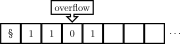
\includegraphics{res/turing_add1_4}
  \caption{A Turing machine}
  \label{fig:Turing machine}
\end{figure}

\begin{defin}
  Let $\mathbb A = (S, δ)$ be a Turing machine. A \emph{configuration}
  of $\mathbb A$ is a triple $(s, j, c) ∈ S × ℕ × A^ℕ$. It reflects
  the current state of $\mathbb A$, the current position of its
  head, and the content of its work-tape.
\end{defin}

A configuration of the form $(\shalt, 0, c)$ is called \emph{halting}. A
\emph{start configuration} is of the form $(\sstart, 0, c)$ such that $c(0) =
\sta$ and there exists an $n ∈ ℕ$ such that $c(i) = \emp$ if and only if $i >
n$. This means that in a start configuration the work-tape reads
\[
  \sta c(1) c(2) … c(n) \emp \emp …
\]
It will be very convenient to identify the finite string $c(1) c(2) … c(n) ∈ ω$
with this tape content. Note however, that albeit every string can be associated
with a tape content, the converse is not true, e.g.
\[
  \sta \zer \zer \one \emp \zer \emp …
\]
is a valid tape content but we cannot interpret it as a finite string in the
alphabet \(\set{\zer, \one}\). Nevertheless, if reference is clear, the symbols \(b_1b_2 … b_n ∈ ω\) shall denote both the string and the tape content
\[
  c(i) :=
    \begin{cases}
      \sta & \text{if } i = 0\\
      b_i  & \text{if } 1 ≤ i ≤ n\\
      \emp & \text{otherwise}
    \end{cases}
\]

\begin{defin}
  Let \((s, j, c)\) and \((s', j', c')\) be configurations of a Turing machine
  \(\mathbb{A} = (S, δ)\). One writes $(s, j, c) \vdash_1 (s', j', c')$ and
  calls $(s', j', c')$ a \emph{successor configuration} of $(s, j, c)$ if there
  exists an $m ∈ \lbrace -1, 0, 1 \rbrace$ such that

  \begin{itemize}
  \item
    $δ(s, c(j)) = (s', c'(j), m)$,
  \item
    $j' = j + m$, and
  \item
    $c'(ℓ) = c(ℓ)$ for all $ℓ ≠ j$.
  \end{itemize}
\end{defin}

This relation makes the set of all configurations of $\mathbb A$ into a directed
graph. A \emph{run} or \emph{computation} of $\mathbb A$ on $x ∈ ω$ is a path in
this directed graph starting at the start configuration $(\sstart, 0, x)$. A run
of $\mathbb A$ on $x$ is \emph{halting} or \emph{complete} if it reaches a
halting configuration $(\shalt, 0, y)$ with \(y ∈ ω\). In this case I write
$\mathbb A (x) = y$.

I will denote Turing machines using listings, where the fact that
$δ_\text{delta} (\state{state}, b) = (\state{state'}, b', m)$ is encoded by
%
\begin{lstlisting}
delta "state" b = ("state'", b', m)
\end{lstlisting}
%
Variables match all possible states or characters in the alphabet
respectively. However, I follow the convention that if an assignment of
variables matches more than one pattern, the first matching pattern is chosen.
This means that
%
\begin{lstlisting}
delta "state" 1 = ("state'", b', m)
delta "state" b = ("state''", b'', m')
\end{lstlisting}
%
should be interpreted as
\[
  δ(s, b) =
  \begin{cases}
    (\state{state'}, b', m) & \text{if } s=\state{state} ∧ b = \one\\
    (\state{state''}, b'', m') & \text{if } s=\state{state} ∧ b ≠ \one
  \end{cases}.
\]
This kind of pattern matching may seem unconventional at first glance but yields
mutually exclusive definitions of the cases and is standardized in the
specifications of the \emph{Haskell 2010} programming language\footnote{see
\url{https://www.haskell.org/onlinereport/haskell2010}}.
See \cref{app:turing} on how to simulate Turing machines using these listings.

\begin{exam}\label{ex:add 1}
    Consider the Turing machine $\mathbb A_\text{add1} = (\lbrace \sstart,
    \shalt, \state{overflow}, \state{return}, \state{error} \rbrace,
    δ_\text{add1})$ that adds $1$ to a (possibly zero-patched) binary
    representation of a natural number $n$. Its transition function is described
    in \cref{lst:add1}.

    The last line of the program ensures, that $δ$ is a total function, as it
    matches all remaining pairs of states and characters and lets the machine
    enter the state $\state{error}$. The complete run of $\mathbb A_\text{add1}$
    on $\one\one\zer\one$---encoding the number \(11\)---can be seen in
    \cref{fig:complete run}.
\end{exam}

\lstinputlisting[float, frame=tb,
                 caption=A Turing machine adding one to the input string,
                 label=lst:add1]{./listings/add1.hs}

\begin{figure*}
    \begin{subfigure}{.5\textwidth}
        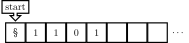
\includegraphics{res/turing_add1_1}
        \caption{$δ(\sstart, \sta) = (s_\text{overflow}, \sta, 1)$}
    \end{subfigure}

    \begin{subfigure}{.5\textwidth}
        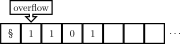
\includegraphics{res/turing_add1_2}
        \caption{$δ(s_\text{overflow}, \one) = (s_\text{overflow}, \one, 1)$}
    \end{subfigure}

    \begin{subfigure}{.5\textwidth}
        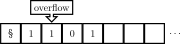
\includegraphics{res/turing_add1_3}
        \caption{$δ(s_\text{overflow}, \one) = (s_\text{overflow}, \one, 1)$}
    \end{subfigure}

    \begin{subfigure}{.5\textwidth}
        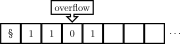
\includegraphics{res/turing_add1_4}
        \caption{$δ(s_\text{overflow}, \zer) = (s_\text{return}, \one, -1)$}
    \end{subfigure}

    \begin{subfigure}{.5\textwidth}
        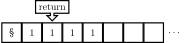
\includegraphics{res/turing_add1_5}
        \caption{$δ(s_\text{return}, \one) = (s_\text{return}, \one, -1)$}
    \end{subfigure}

    \begin{subfigure}{.5\textwidth}
        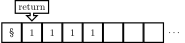
\includegraphics{res/turing_add1_6}
        \caption{$δ(s_\text{return}, \one) = (s_\text{return}, \one, -1)$}
    \end{subfigure}

    \begin{subfigure}{.5\textwidth}
        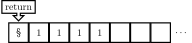
\includegraphics{res/turing_add1_7}
        \caption{$δ(s_\text{return}, \sta) = (s_\text{halt}, \sta, 0)$}
    \end{subfigure}

    \begin{subfigure}{.5\textwidth}
        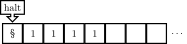
\includegraphics{res/turing_add1_8}
        \caption{$δ(s_\text{halt}, \sta) = (s_\text{halt}, \sta, 0)$}
    \end{subfigure}

    \caption{The complete run of $\mathbb A_\text{add1}$ on $\one\one\zer\one$}
    \label{fig:complete run}
\end{figure*}

\begin{defin}
    Let $\mathbb A$ be a Turing machine.

    \begin{thmlist}
        \item
          $\mathbb A$ \emph{computes} the partial function that maps each
          $x$ with a complete run to $\mathbb A(x)$ and is undefined for all
          other strings.
        \item
          $\mathbb A$ \emph{accepts} all $x$ such that
          $\mathbb A(x) = \one$ and \emph{rejects} them if
          $\mathbb A(x) = \zer$.
        \item
          A partial function on $\lbrace \zer, \one \rbrace^*$ is
          \emph{computable} if there exists a Turing machine computing it.
          Sometimes computable functions are referred to as \emph{recursive} or
          \emph{efficient} functions.
        \item
          A subset of $ω = \lbrace \zer, \one \rbrace^*$, i.e.\ a problem, is
          \emph{decidable} if there exists a Turing machine computing its
          characteristic function.
        \item
          A problem is called \emph{semi-decidable} or \emph{computably
          enumerable} if there exists a Turing machine accepting precisely the
          elements of the problem.
    \end{thmlist}
\end{defin}

The last item of the definition above means that a problem is
semi-decidable if there is a Turing machine affirming membership of the
corresponding set but it might not be able to refute membership.

\begin{exam}\label{ex:finite problems are decidable}
  Let \(Q\) be a finite problem then \(Q\) is decidable. To see this let \(n\)
  be the maximal length of a string in \(Q\) and construct a Turing machine
  \(\mathbb{A}\) with the states
  \[
    S = \set{\sstart, \shalt, \state{accept}, \state{reject}} \sqcup
    \set{s_{b_1…b_k} \mid b_1…b_k ∈ ω \text{ for } 0 ≤ k ≤ n},
  \]
  where \(\sqcup\) denotes the disjoint union. As for the transition function
  \(δ\), we define
  \begin{align*}
    δ(\sstart, §)        &:= (s_λ, §, 1)\\
    δ(s_{b_1…b_k}, \one) &:=
      \begin{cases}
        (s_{b_1…b_k\one}, \one, 1) & \text{if } k < n\\
        (\state{reject}, \emp, -1) & \text{otherwise}
      \end{cases}\\
    δ(s_{b_1…b_k}, \zer) &:=
    \begin{cases}
      (s_{b_1…b_k\zer}, \zer, 1) & \text{if } k < n\\
      (\state{reject}, \emp, -1) & \text{otherwise}
    \end{cases}\\
    δ(s_{b_1…b_k}, \emp) &:=
      \begin{cases}
        (\state{accept}, \emp, -1) & \text{if } b_1…b_k ∈ Q\\
        (\state{reject}, \emp, -1) & \text{if } b_1…b_k \not\in Q\\
      \end{cases},
  \end{align*}
  where the schemes in the last three lines should be understood as one
  instruction per string \(b_1…b_k ∈ ω\) for \(1 ≤ k ≤ n\). This way we obtain \[
    1 + 3 \sum_{i=0}^n 2^i = 1 + 3 \left(2^{n + 1} - 1\right)
  \]
  equations for \(δ\). The idea of this machine is that it enters the state that
  corresponds to the string on the tape that the machine has read so far. Now
  one of three things can happen:
  \begin{itemize}
    \item Either the input string continues and we have read less than \(n\)
    symbols so far, then the machine continues reading (first case of lines 2
    and 3); or
    \item the machine reads a blank symbol \(\emp\), then we must check if the
    string is in \(Q\) and accept or reject accordingly (line 4); or
    \item we have already read \(n\) symbols, then we can reject for sure as
    \(Q\) contains no string with more than \(n\) symbols (second case of lines
    2 and 3).
  \end{itemize}

  It is now easy to extend \(δ\) into a total function \(S \times A → S \times A
  \times \set{-1, 0, 1}\) such that once \(\mathbb{A}\) reaches
  \(\state{accept}\), the machine clears the tape except for a single \(\one\),
  and if  \(\mathbb{A}\) reaches \(\state{reject}\), it clears the tape except
  for a single \(\zer\), and halts.
\end{exam}

Note that the construction above fails if \(Q\) is infinite because in this case
the set of states \(S\) is infinite. However, if \(Q\) is co-infinite we can
exchange \(\state{accept}\) and \(\state{reject}\) in the construction above to
obtain a Turing machine deciding \(Q\). In \cref{pro:Posts theorem} we will see
that the complements of decidable sets are decidable in general.

Before we can prove that further sets are decidable we need a bit more theory of
computable functions.

\begin{lem}\label{lem:composition of Turing machines}
  Let $\mathbb A_1 = (S_1, δ_1)$ and $\mathbb A_2 = (S_2, δ_2)$ be Turing
  machines computing $f_1: D_1 → ω$ and $f_2: D_2 → ω$ respectively ($D_1, D_2
  \subseteq ω$). Then there exists a Turing machine $\mathbb A_{f_2 \circ f_1}$
  computing the partial function $f_2 \circ f_1: D_1 ∩ f_1^{-1}(D_2) → ω$
  obtained by composing $f_1$ and $f_2$.
\end{lem}
\begin{proof}
  If \(\sstart = \shalt\) then machine \(\mathbb{A}_1\) and machine
  \(\mathbb{A}_2\) compute the identity function on \(ω\) and the claim is
  trivial. Similarly, if \(δ_1(\sstart, \sta) = (\shalt, \sta, 0)\), then
  \(\mathbb{A}_1\) computes the identity and the claim is proven by setting
  \(\mathbb{A}_{f_2 \circ f_1} = \mathbb{A}_2\)

  We can therefore assume that we are not in these degenerate cases and
  construct $\mathbb A_{f_2 \circ f_1}$ from $\mathbb A_1$ and $\mathbb A_2$ as
  follows: Let $S_1' := S_1 \setminus \set{\sstart, \shalt}$ and $S_2' := S_2
  \setminus \set{\sstart, \shalt}$, then set $S = \set{\sstart, \shalt} \sqcup
  S_1' \sqcup S_2' \sqcup \set{\state{compose}}$, where $\sqcup$ denotes the
  disjoint union. Now for a state \(s ∈ S\) and a symbol $b ∈ A$ we define
  %
  \begin{align*}
    δ (s, b) &:=
      \begin{cases}
        δ_1 (s, b) & \text{if } s ∈ S_1' ∪ \set\sstart \\
        (\state{compose}, b, m) & \text{if } s ∈ S_1 \text{ and } δ_1(s, b) = (\shalt, b', m)\\
        δ_2 (s, b) & \text{if } s ∈ S_2' ∪ \set\shalt \\
        δ_2 (\sstart, b) & \text{if } s = \state{compose}
      \end{cases}
  \end{align*}
  %
  Then $\mathbb A_{f_2 \circ f_1} = (S, δ)$ computes $f_2 \circ f_1$ because $δ$
  is defined to first run the program of $\mathbb A_1$ and if this machine
  reaches a halting state run $\mathbb A_2$.
\end{proof}

\begin{exam}
    One can encode a natural number $n$

    \begin{exlist}
    \item\label{ex:tally encoding}
      in tally notation
      \begin{align*}
        n & ↦ \underbrace{\one…\one}_{n\text{-times}},
          \quad \text{if } n > 0, \\
        0 & ↦ λ;
      \end{align*}
    \item
      by its binary representation
      \begin{align*}
          n = 2^k + \sum_{i = 0}^{k-1} b_i 2^i & ↦ b_0…b_{k-1}\one,
            \quad \text{if } n > 0\\
                                             0 & ↦ \zer; \text{ or}
      \end{align*}
    \item\label{ex:omega encoding}
      by a shifted and truncated form of its binary representation
      \begin{align*}
        n = 1 + \sum_{i = 0}^k b_i 2^i & ↦ b_0…b_k, \quad \text{if } n > 0,\\
                                     0 & ↦ λ.
      \end{align*}
      In other words, $n$ is mapped to the $n$-th string if one orders $\lbrace
      \zer, \one \rbrace^*$ lexicographically. I will write \(<_{lex}\) for the
      lexicographical ordering of \(ω = \set{\zer, \one}^*\).  As \(ω\)
      traditionally denotes the non-negative integers in the fields of logic and
      especially set theory, this last encoding is the reason why I am using the
      symbol \(ω\) to denote the set of finite strings \(\set{\zer, \one}^*\).
    \end{exlist}

    In either case the set obtained by encoding $ℕ$ is easily seen to be
    decidable. In the first case, check that the string contains only copies
    of the bit $\one$. Indeed, this can be achieved by the Turing machine
    \[
      \mathbb A_\text{tally} =
        ( \lbrace \sstart, \shalt, \scheck, \state{accept}, \state{reject},
          \state{rejectMR}, \state{error} \rbrace, δ),
    \]
    whose transition function is displayed in \cref{lst:tally encoding}. In the
    second case it suffices to check that the string has length $1$ or ends in a
    $\one$, and in the third case every string is accepted.
\end{exam}

\lstinputlisting[float, frame=tb,
                 caption=A Turing machine checking whether the input is tally-encoded,
                 label=lst:tally encoding]{./listings/tally.hs}

\begin{rem}
  Let \(Q_0\) be a decidable problem and \(Q \subseteq Q_0\) a subset. If there
  exists a Turing machine \(\mathbb{A}\) that upon receiving \(x ∈ Q_0\) as
  input decides whether \(x ∈ Q\), then \(Q\) is decidable. In other words, if
  one can decide a problem relative to a decidable problem then the initial
  problem is globally decidable. To obtain a Turing machine deciding \(Q\) we
  first run the Turing machine deciding \(Q_0\) and reject \(x\) if \(Q_0(x) =
  \zer\) otherwise we run \(\mathbb{A}\) on \(x\).
\end{rem}

Taking another look at the definition of computability, one sees that only
functions in one argument defined on subsets of $ω$, mapping to subsets of $ω$
can be computable. However, one can easily extend this to functions on multiple
arguments, by encoding tuples in $ω \times ω$ by elements of $ω$ in such a way,
that the projections $p_i: \enc{(x_1, x_2)} ↦ x_i$  for $i ∈ \lbrace 0, 1
\rbrace$ are computable. This means, there are injective pairing functions $ω^2
→ ω$ and Turing machines $\mathbb P_1, \mathbb P_2$ computing $p_1$ or $p_2$
respectively.

\begin{exam}[Pairing functions]
  \begin{exlist}
    \item\label{ex:tally pairing}
    Using tally notation (cf.~\cref{ex:tally encoding}) on can encode $(n, m) ∈
    ℕ^2$ by
    \[
      ⟨\enc{n}, \enc{m}⟩ = \underbrace{\one … \one}_{n\text{-times}} \zer \underbrace{\one … \one}_{m\text{-times}}.
    \]
    The machine \(\mathbb{P}_1\) clears everything after the first \(\zer\) on
    the tape and \(\mathbb{P}_2\) deletes everything up to the first zero and
    then moves the second block of \(\one\)-s cell by cell from left to right.

    \item\label{ex:total pairing}
    A simple pairing function encodes the pair $(b_1b_2…b_n, c_1c_2…c_m) ∈ ω^2$
    by
    \[
      ⟨b_1b_2…b_n, c_1c_2…c_m⟩ = b_1b_1b_2b_2…b_nb_n \; \zer\one \; c_1c_2…c_m.
    \]
    In this encoding the second projection is obtained completely analogously as
    in the previous example. As for the first projection, the machine
    \(\mathbb{P}_1\) first moves to the right, deleting every second symbol
    until it reaches the substring \(\zer\one\) indicating the end of the first
    component. At this point, the machine deletes all symbols to its right until
    it reaches the first blank symbol and returns to the left until it reads
    \(b_n\) in cell \(2n - 1\). The tape will now look like the one in
    \cref{fig:total pairing non empty}.

    Next it starts shifting the content of all cells one cell to the left until
    it reaches the end of tape symbol \(\sta\) (cf.~\cref{fig:total pairing
    shift left 1} and c). The machine can find the end of the string by moving
    to the right until it finds two consecutive blank cells (cf.~\cref{fig:total
    pairing double blank}). At this point the whole process starts over, except
    when shifting left, the machine must check, if the cell it wants to write to
    is empty. If it is not empty, it starts moving right again to find two
    consecutive blank cells. The process stops if it reads two consecutive blank
    cells before reading a single blank cell.
  \end{exlist}
\end{exam}

\begin{figure*}
    \begin{subfigure}{.7\textwidth}
        \includegraphics{res/turing_p1_1}
        \caption{The machine finds the first non-empty cell.}%
        \label{fig:total pairing non empty}
    \end{subfigure}

    \begin{subfigure}{.7\textwidth}
        \includegraphics{res/turing_p1_2}
        \caption{The machine shifts the content of each cell one cell to the
                 left …}%
        \label{fig:total pairing shift left 1}
    \end{subfigure}

    \begin{subfigure}{.7\textwidth}
        \includegraphics{res/turing_p1_3}
        \caption{… until it reaches the end of tape symbol \(\sta\).}%
        \label{fig:total pairing shift left 2}
    \end{subfigure}

    \begin{subfigure}{.7\textwidth}
        \includegraphics{res/turing_p1_4}
        \caption{The machine finds two consecutive blank cells and starts
                 over.}%
        \label{fig:total pairing double blank}
    \end{subfigure}

    \caption{A schematic run of the first projection associated to the pairing
             function in \cref{ex:total pairing}}%
    \label{fig:pairing function}
\end{figure*}

By applying a pairing function iteratively one obtains an $n$-ary pairing
function. The projections need to be composed accordingly. For example
\[
  (x_1, x_2, x_3) ↦ ⟨x_1, ⟨x_2, x_3⟩⟩
\]
yields a ternary pairing function and $π_1\circ π_2$ is the projection onto
$x_2$. Using any of the pairing functions above, one can consider $n$-ary
computable functions by providing the encoded pair $⟨x_1, x_2, …, x_n⟩$ as the
single argument of a Turing machine $\mathbb A$. If the context is clear, I will
write $\mathbb A(\seq{x})$ in this situation. Furthermore, these pairing
functions allow us to define decidable relations on \(ω^n\).

\begin{defin}
  Let \(R \subseteq ω^n\) be an \(n\)-ary relation on \(ω\). Then \(R\) is
  called (\emph{semi-})\emph{decidable} if the set
  \[
    \set{⟨\seq{x}⟩ \mid \seq{x} ∈ ω, R(\seq{x})}
  \]
  is a (semi-)decidable subset of \(ω\).
\end{defin}

When trying to find solution of equations or witnesses for relations the concept
of \emph{effective search} is very important. In the theory of computability it
is modelled by a minimization operator.

\begin{defin}
  Let \(R \subset ω^2\) be a semi-decidable relation. We say \(f: D_R → ω\) is
  obtained from \(R\) via \emph{minimization} and write
  \[
    f(x) = μy: R(x, y)
  \]
  if
  \[
    D_R = \set{x ∈ ω \mid ∃ y ∈ ω : R(x, y)},
  \]
  there exists a Turing machine \(\mathbb{A}\) semi-deciding \(R\), such that
  for all \(x ∈ D_R\) the machine \(\mathbb{A}\) can refute \(R(x, y)\), i.e.\
  \(\mathbb{A}(x, y) = \zer\), for all \(y <_{lex} f(x)\), and \(R(x, f(x))\)
  holds.
\end{defin}

\begin{lem}\label{lem:minimization}
  If \(f: D_R → ω\) is obtained from a semi-decidable relation \(R \subset ω^2\)
  via minimization, then \(f\) is computable.
\end{lem}
\begin{proof}
  Let \(x ∈ D_R\). We will start by trying whether the empty string \(λ\)
  satisfies \(R(x, λ)\). If this is the case, then \(f(x) = λ\) and we are done.
  Otherwise, the Turing machine semi-deciding \(R\) can refute \(R(x, λ)\) and
  we move on to try the next string in lexicographical order. By definition of
  \(D\), there exists a string \(y ∈ ω\) such that \(R(x, y)\) holds and this
  string will appear in our listing of \(ω\) after finitely many steps. Thus,
  \(f\) is computable.

  More formally, such a Turing machine computing \(f\) can be obtained as
  follows. First apply a Turing machine that transforms a string \(b_1b_2…b_n ∈
  ω\) into the tape content
  \[
    \sta \; b_1 \emp \emp \; b_2 \emp \emp … b_n
  \]

  Starting to count at index \(0\), the cells whose index is congruent \(2\)
  modulo \(3\) encode the empty string \(λ\). We apply a Turing machine that
  computes \(⟨b_1b_2…b_n, λ⟩\) from the cells whose index is congruent \(1\) or
  \(2\) modulo \(3\) and writes only to the cells whose index is congruent \(0\)
  modulo \(3\). Then the tape will read something like
  \[
    \sta \; b_1 \emp b_1 \; b_2 \emp b_1 \; b_3 \emp b_2 ….
  \]

  Now transform the Turing machine \(\mathbb{A}_R\) used in the definition of
  minimization into one that only uses cells congruent \(0\) modulo \(3\) and
  apply it to the tape content. If \(\mathbb{A}_R\) accepts we have found
  \(f(x)\).

  Otherwise, we use a slight modification of the Turing machine of \cref{ex:add
  1}, to obtain a Turing machine that upon receiving \(x\) as input, outputs the
  next string in lexicographical order and uses only cells whose index is
  congruent \(2\) modulo \(3\). At this point, we start the next iteration.
\end{proof}

We are now able to state equivalent definitions of decidable and semi-decidable
sets.

\begin{pro}\label{pro:characterizations of ce sets}
  Let \(Q\) be a problem. The following are equivalent.
  \begin{thmlist}
    \item \(Q\) is semi-decidable.
    \item \(Q\) is the domain of a partial computable function.
    \item There exists a decidable relation \(R \subseteq ω^2\) such that
    \[
      x ∈ Q \quad ⇔ \quad ∃ y ∈ ω : R(x, y)
    \]
  \end{thmlist}
\end{pro}
\begin{proof}
  \emph{(i) \(⇒\) (ii):} Let \(\mathbb{A}\) be a Turing machine witnessing that
  \(Q\) is semi-decidable. Then \(\mathbb{A}\) halts on all \(x ∈ Q\) and
  returns \(\one\). If on the other hand \(x \not\in Q\) then \(\mathbb{A}\)
  outputs an arbitrary string \(y ≠ \one\) or does not halt on \(x\).

  Consider the Turing machine \(\mathbb{A}_{check1}\) defined in \cref{lst:check
  one}. It outputs \(\one\) on input \(\one\) and does not halt on any other
  input. The machine obtained by composing \(\mathbb{A}\) and
  \(\mathbb{A}_{check1}\) does halt on \(x\) if and only if \(x ∈ Q\).

  \emph{(ii) \(⇒\) (iii):} Let \(\mathbb{A}\) be a Turing machine computing the
  partial computable function, whose domain is \(Q\). For each integer \(n ∈
  ℕ\), I denote by \(\mathbb{A}_n\) the set of all strings \(x := b_1…b_k ∈ ω\)
  such that \(k ≤ n\) and \(\mathbb{A}\) halts on \(x\) in at most \(n\) steps
  of the computation.

  As \(|\mathbb{A}_n| ≤ 2^n\) is finite for all \(n ∈ ℕ\), the sets
  \(\mathbb{A}_n\) are decidable by \cref{ex:finite problems are decidable}.
  Using induction on \(n\), we see that the relation
  \[
    R(x, \enc{n}) \quad :⇔ \quad x ∈ \mathbb{A}_n
  \]
  is decidable by continuing the execution of \(\mathbb{A}\) for one more step.
  Finally, we obtain
  \[
    x ∈ Q \quad ⇔ \quad ∃ y ∈ ω: R(x, y),
  \]
  as claimed.

  \emph{(iii) \(⇒\) (i):} By \cref{lem:minimization} the function \(f(x) = μy :
  R(x, y)\) is computable. Compose \(f\) with a function that returns \(\one\)
  on all inputs to obtain a computable function that outputs \(\one\) for all
  \(x ∈ Q\) and is undefined otherwise.
\end{proof}

\lstinputlisting[float, frame=tb,
                 caption=A Turing machine that halts and accepts only on input \(\one\),
                 label=lst:check one]{./listings/check1.hs}

The following proposition---which is sometimes referred to as \emph{Post's
theorem}---is intuitively clear. It states that if we have an algorithm
that can affirm membership of a problem \(Q\) and if there is an algorithm that
can refute membership, then we can decide \(Q\). However, a formal proof is
technically quite intricate.

\begin{pro}\label{pro:Posts theorem}
  Let \(Q\) be a problem. Then \(Q\) is decidable if and only if \(Q\) and \(ω
  \setminus Q\) are semi-decidable.
\end{pro}
\begin{proof}
  Assume \(Q\) to be decidable by the Turing machine \(\mathbb{A}\), then \(Q\)
  is semi-decidable in particular. Now compose \(\mathbb{A}\) with a Turing
  machine \(\mathbb{B}\) with the property \(\mathbb{B}(\one) = \zer\) and
  \(\mathbb{B}(\zer) = \one\). One obtains a Turing machine deciding the
  complement of \(Q\) and \(ω \setminus Q\) is thus semi-decidable, as claimed.

  If on the other hand, \(Q\) and \(ω \setminus Q\) are semi-decidable, then
  there are Turing machines \(\mathbb{A}\) and \(\mathbb{A}^c\) semi-deciding
  \(Q\) and \(ω \setminus Q\) respectively. By \cref{pro:characterizations of ce
  sets} we may assume that these machines only halt on strings contained in
  \(Q\) or \(ω \setminus Q\) respectively, and that their only output is
  \(\one\).

  We want to run these Turing machines in parallel. As each string \(x ∈ ω\) is
  either contained in \(Q\) or not, one of these machines will halt and output
  \(\one\), indicating whether \(x\) belongs to \(Q\) or not.

  To this end, construct a Turing machine \(\mathbb{A}_{copy4}\) that transforms
  an input string \(x_1x_2 … x_n ∈ ω\) to
  \[
    \one\zer\one\zer \zer x_1 \zer x_1 \zer x_2 \zer x_2 … \zer x_n \zer x_n.
  \]
  Starting to count at \(1\), cells with an index \(i \equiv 1 \mod 4\) indicate
  if the head of machine \(\mathbb{A}\) is currently reading the cell with index
  \(i + 1\), in this case a \(\one\) is placed inside this cell, \(\zer\)
  otherwise; cells with an index \(i \equiv 2 \mod 4\) represent the the tape
  of machine \(\mathbb{A}\); and cells with indices congruent \(3\) or \(0\)
  modulo \(4\) represent the corresponding information for machine
  \(\mathbb{A}^c\). The first block of \(4\) bits represents the ends of the
  tapes of machine \(\mathbb{A}\) and \(\mathbb{A}^c\) respectively.

  Now construct a Turing machine \(\mathbb{D}\) whose states \(S = S_1 \times
  S_2 \times S_{aux}\) are triples of states of machine \(\mathbb{A}\), states
  of machine \(\mathbb{A}^c\), and some auxiliary states \(S_{aux}\).

  Say machine \(\mathbb{D}\) is in state \((s_1, s_2, s_a)\). At odd stages of
  the computation of \(\mathbb{D}\) the head rests at the end of tape symbol
  \(§\) and starts moving to the right until it finds the first \(\one\) in a
  cell with an index \(i \equiv 1 \mod 4\). All computation steps necessary for
  this will only effect \(s_a\) and preserve \(s_1\) and \(s_2\).
  Next the machine will mark cell \(i\) with \(\zer\) and will then carry out
  one step of the computation of \(\mathbb{A}\), reading the cell with index \(i
  + 1\) and writing in one of the cells with indices \(i - 3, i + 1\) and \(i +
  5\). Thereby the state \(s_1\) will be changed to the state dictated by the
  transition function of machine \(\mathbb{A}\).
  Finally, the head moves one cell to the left, marks by writing a \(\one\) the
  last position of its head, and moves back to the end of the tape.

  Add even stages the head moves to the right until it finds the first \(\one\)
  in a cell with an index \(i \equiv 3 \mod 4\) and carry out the analogous
  steps for machine \(\mathbb{A}^c\) as in the even case.

  At some point either the computation of \(\mathbb{A}\) or the one of
  \(\mathbb{A}^c\) will halt. Then \(\mathbb{D}\) has reached a state where
  either the first or the second component of \((s_1, s_2, s_a) ∈ S\) is a
  halting state. Then \(\mathbb{D}\) can clear the tape and write \(\one\) or
  \(\zer\) to the cell with index \(1\) to indicate whether \(s_1 = \shalt\) or
  \(s_2\) does.
\end{proof}

\subsection{Church-Turing thesis and the halting problem}
% ██   ██  █████  ██   ████████ ██ ███    ██  ██████      ██████
% ██   ██ ██   ██ ██      ██    ██ ████   ██ ██           ██   ██
% ███████ ███████ ██      ██    ██ ██ ██  ██ ██   ███     ██████
% ██   ██ ██   ██ ██      ██    ██ ██  ██ ██ ██    ██     ██
% ██   ██ ██   ██ ███████ ██    ██ ██   ████  ██████      ██ ██

In the remainder of this thesis I will make use of the following
meta-mathematical thesis. That cannot be mathematically proven but has been
heuristically justified for all of the generally accepted\footnote{The
interested reader should find the comment \cite{Davis2006} on hyper-computation
by Davis quite revealing.} formalizations of computation. It allows one to state
properties of computability without referring to a specific model.

\begin{quote}
  \textsc{Churh-Turing thesis.} The class of intuitively computable
  functions coincides with the class of all Turing computable functions.
\end{quote}

In his foundational paper~\cite{Turing1936} Turing proved a crucial result for
the whole field of computability theory and its practical applications. He noted
\begin{quote}
  It is possible to invent a single machine which can be used to compute any
  computable sequence.
\end{quote}
This may seem not surprising to the reader of the twenty-first century, who is
used to being surrounded by machines that can carry out nearly all tasks
imaginable, but the insight, that it is possible to build a single machine that
can carry out all computations, can hardly be overestimated.

\begin{thm}
    There exists a Turing machine $\mathbb U$ that computes upon receiving
    the tuple $⟨\ulcorner \mathbb A \urcorner, x⟩$ as input, the output of
    Turing machine $\mathbb A$ on $x$ i.e.
    \[
      \mathbb U(\ulcorner \mathbb A \urcorner, x) = y \Leftrightarrow
        \mathbb A (x) = y
    \]
\end{thm}

As a last task of this section we want to find a set \(\mathcal{K} \subseteq ω\)
that is semi-decidable but not decidable. It will be the key ingredient in the
task of settling Hilbert's tenth problem. Note that it is not hard to see that
an undecidable problem exists, as there are only countably many Turing machines
but uncountably many problems. However, to find such a set within the
semi-decidable ones we turn our attention to a problem that quite naturally
arises in computability theory.
\begin{quote}
  \textsc{halting problem.} Given a machine $\mathbb A$ and a string $x$. Does
  $\mathbb A$ halt on $x$?
\end{quote}
The contradiction to the existence of a Turing machine deciding this problem is
obtained by a diagonalization technique that is also present in Cantor's proof
that the power set of the integers is uncountable or Russel's paradox.

\begin{thm}
    The halting problem is undecidable.
\end{thm}
\begin{proof}
    Assume there exists a Turing machine $\mathbb B$ that decides the
    halting problem i.e.~for all Turing machines $\mathbb A$ and all
    strings $x$

    \[ \mathbb B(\enc{\mathbb A}, x) =
    \begin{cases}
      \one  & \text{if } \mathbb A \text{ halts on } x\\
      \zer  & \text{if } \mathbb A \text{ does not halt on } x
    \end{cases}\]

    Now using $\mathbb B$ construct a Turing machine $\mathbb B'$ that
    simulates $\mathbb B(\enc{\mathbb A}, \enc{\mathbb A})$ on its input
    $\enc{\mathbb A}$ and enters an infinite loop if
    $\mathbb B(\enc{\mathbb A}, \enc{\mathbb A}) = \zer$. Expressed more
    formally this means
    \[
      \mathbb B' \text{ halts on } \enc{\mathbb A} \quad ⇔ \quad
      \mathbb A \text{ does not halts on } \enc{\mathbb A}.
    \]
    Setting $\mathbb A = \mathbb B'$ yields the desired contradiction.
\end{proof}

For a more detailed proof of theorem fact and lot more information on
computability see \cite{Cooper2004}. As the halting problem is undecidable the
\emph{halting set} defined by
\[
 \mathcal{K} = \set{⟨\enc{\mathbb A}, x⟩ \mid \mathbb A \text{ halts on } x}
\]
is undecidable. However, using the universal Turing machine it is seen to be
semi-decidable.

\begin{cor}
  The halting set is semi-decidable but not decidable.
\end{cor}

\begin{rem}
  Note that the halting set contains the information of \emph{all}
  semi-decidable sets in the sense that given a semi-decidable set \(Q\), there
  is a total computable function \(f: ω → ω\) such that
  \begin{equation}\label{eq:m reducibility}
    x ∈ Q \quad ⇔ \quad f(x) ∈ \mathcal{K}.
  \end{equation}

  Indeed, since \(Q\) is semi-decidable, by \cref{pro:characterizations of ce
  sets} there exists a Turing machine \(\mathbb{A}\) that halts on \(x\) if and
  if \(x ∈ Q\). This means that
  \[
    x ∈ Q \quad ⇔ \quad ⟨\enc{\mathbb{A}}, x⟩ ∈ \mathcal{K}.
  \]
  Setting \(f(x) := ⟨\enc{\mathbb{A}}, x⟩\) yields the claim.
\end{rem}

We say a problem \(Q\) is \emph{many-one reducible} to a second problem \(Q'\)
if there exists a total computable function \(f: ω → ω\) as in \eqref{eq:m
reducibility}. One writes \(Q ≤_m Q'\) in this situation. In the remark we have
seen that all semi-decidable sets are many-one reducible to \(\mathcal{K}\). The
key step in settling Hilbert's tenth problem is proving that \(\mathcal{K}\) is
many-one reducible to a collection of sets which are definable by polynomial
equations. This suffices to prove the undecidability of Hilbert's tenth problem,
since we have the following proposition.

\begin{pro}\label{pro:m reducibility and decidability}
  Let \(Q, Q' \subseteq ω\) be problems such that \(Q ≤_m Q'\). Then if \(Q'\)
  is decidable, so is \(Q\).
\end{pro}
\begin{proof}
  Let \(f: Q → Q'\) be the computable function witnessing many-one reducibility
  of \(Q\) to \(Q'\). Since the characteristic function \(χ_{Q'}: ω → ω\) is
  computable, the composition \(g := χ_{Q'} \circ f\) is a total computable
  function with the property
  \[
    g(x) =
      \begin{cases}
        \one & \text{if } x ∈ Q\\
        \zer & \text{otherwise}
      \end{cases}
  \]
  and \(Q\) is decidable.
\end{proof}
